% Build on the outline below.  Cite by using \citep{Author2016} to add a
% parenthetical citation; use \citet{Author2016} to get a textual cite like
% this: Author (2016). 

\section{Examine All Available Data}

examine as much relevant evidence as possible

discuss Figure \ref{F:t2_pooled}

discuss Figure \ref{F:t2_by_survey}


\begin{figure}[htbp] 
  \caption{Local Inequality and the Perception of America as Divided into `Haves' and `Have-Nots': Results Using All Available Data}
  \label{F:t2_pooled}
  \begin{center}
    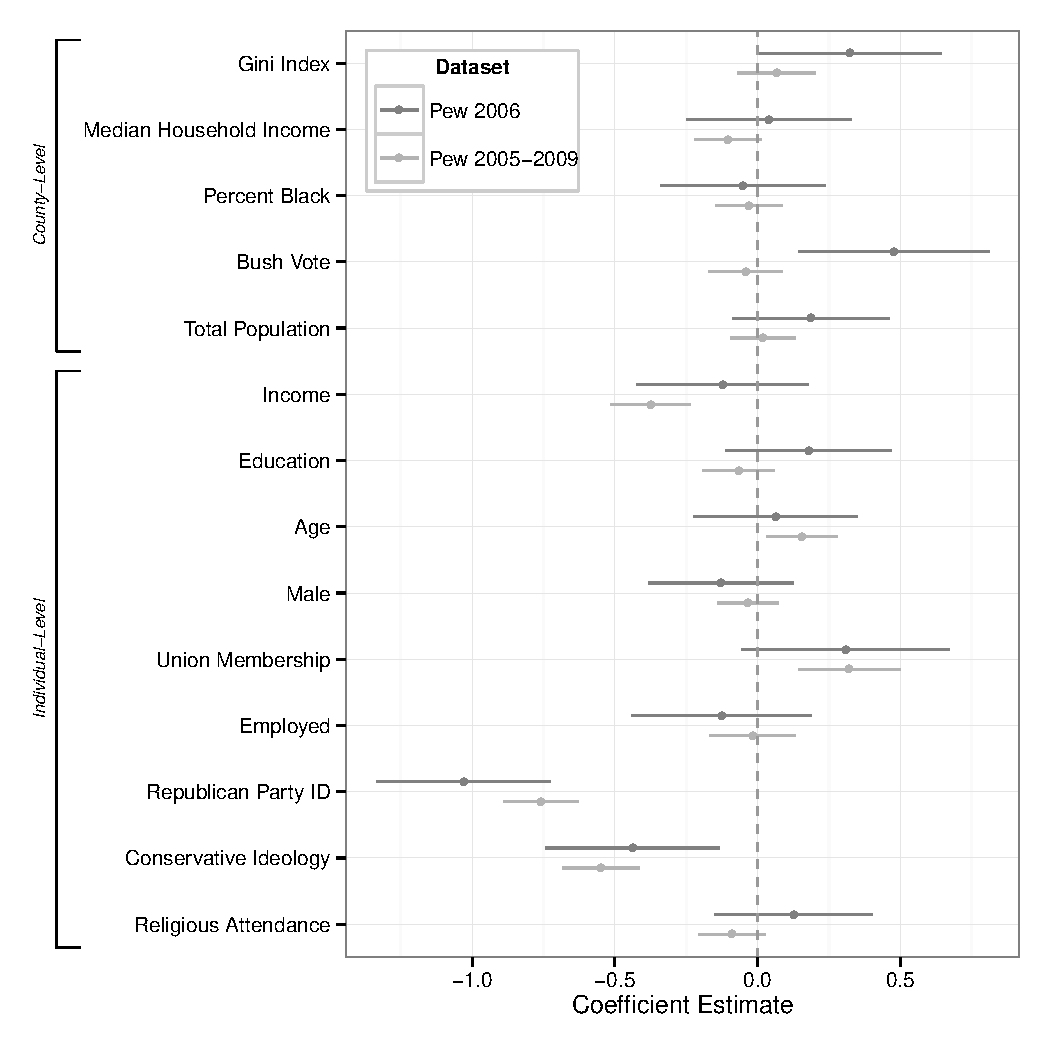
\includegraphics[width=5.25in]{../figures/03_examine_all_available_data_t2.pdf}
  \end{center}
  \begin{footnotesize}
  \begin{tabular}{p{.1in} p{5.1in}}
  & \emph{Notes}: Results from replications of the model presented in Table 2 of \citet{Newman2015} on the 2006 Pew survey analyzed in that article and on pooled data from the six Pew surveys that included the same item and were conducted in the time period the article examines.  The statistically significant result for county income inequality in the 2006 survey presented in that article is not evident when all of the available data are examined.
  \end{tabular}
  \end{footnotesize}
\end{figure}

\begin{figure}[htbp] 
  \caption{Local Inequality and the Perception of America as Divided into `Haves' and `Have-Nots': Results Using Each Available Dataset}
  \label{F:t2_by_survey}
  \begin{center}
    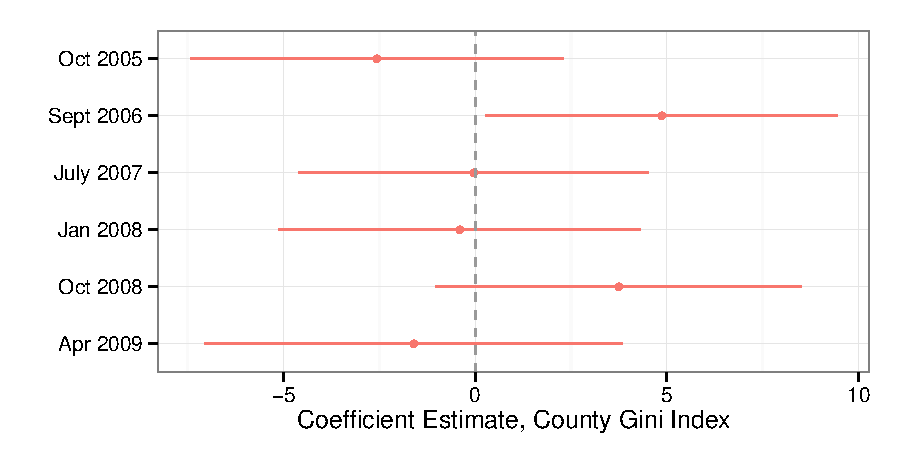
\includegraphics[width=5.25in]{../figures/03_examine_all_available_data_t2_by_survey.pdf}
  \end{center}
  \begin{footnotesize}
  \begin{tabular}{p{.1in} p{5.1in}}
  & \emph{Notes}: Results for county income inequality from replications of the model presented in Table 2 of \citet{Newman2015} on data from each of six available surveys conducted in the in the time period examined in \citet{Newman2015}.  Of the six surveys, the only one that yields a statistically significant result is the 2006 survey presented in that article.
  \end{tabular}
  \end{footnotesize}
\end{figure}



